\section{Selección y muestreo de keyframes}
Un problema al tratar con optimización a tiempo real es la cantidad de datos contra el tiempo necesario para procesarlos. La cámara equipada da lugar a un flujo constante de imágenes, llamadas fotogramas o \textit{frames}, de forma tan frecuente que resulta inviable procesarlas todas. Debido a esto, se escogen de forma estratégica qué fotogramas van a ser utilizados para la optimización. Los mismos son llamados fotogramas clave, de ahora en adelante \textit{keyframes}.

La selección de keyframes es categorizada por \cite{robotics12030088} en tres tipos principales: basados en métodos probabilísticos, basados en heurísticas o basados en métodos de aprendizaje.

En el marco de este trabajo, dado un fotograma nuevo se clasifica como keyframe si cumple con un criterio de covisibilidad con el keyframe anterior menor a una cota superior. Esto quiere decir que la información que representa respecto del último keyframe es lo suficientemente nueva.

Para obtener la covisibilidad, se necesita primero calcular la visibilidad estimada de las gaussianas en ambos fotogramas por separado. En cada uno, se identifica qué gaussianas son utilizadas para renderizarlo bajo la representación actual del mundo, observando si su contribución es significativa. Luego, se utiliza una fórmula de Intersección Sobre Unión (Intersection over Union, abreviado IoE) para calcular el ratio:

Sea $G_i$ el conjunto de gaussianas que se consideran visibles,
$$
IoE (G_1, G_2) = \frac{|G_1 \cap G_2|}{|G_1 \cup G_2|} 
$$

Observemos que el denominador no debería anularse, ya que el keyframe anterior debería tener al menos una gaussiana representándolo tras los debidos pasos de optimización.



Ahora, para optimizar sobre ese conjunto de keyframes se toma una muestra que incluya el último. Esto es para no utilizar el conjunto entero, disminuyendo costos de cómputo, pero representando satisfactoriamente el espacio de interés.

Este muestreo se puede realizar de distintos modos, como utilizando distribuciones probabilísticas, tomando siempre los últimos $n$ keyframes o una combinación de ambas, muestreando n con una distribución sobre una ventana de los últimos k keyframes. 



En este trabajo, el muestreo se realizó con una distribución beta-binomial. La misma se define a partir de tres parámetros: $n$, $\alpha$ y $\beta$, y consiste en una distribución binomial de probabilidad $p$, donde $p \sim Beta(\alpha, \beta)$. De este modo, se puede interpretar como muestrear enteros $0$ a $n$ sobre una curva con forma de la distribución beta correspondiente a los parámetros. 

\begin{figure}[H]
    \centering
    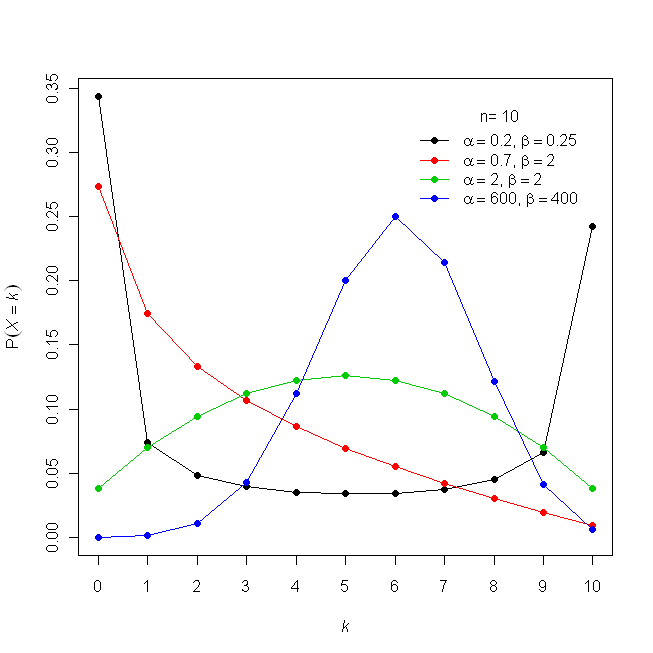
\includegraphics[width=0.8\linewidth]{../imagenes_marco_teorico/Beta-binomial_distribution.png}
    \caption{Distintas combinaciones de $\alpha$ y $\beta$ en la distribución beta binomial para n=10. Con $\alpha = 0.7$ y $\beta=2$ la distribución favorece los valores más bajos con un decaimiento hacia los más altos.}
\end{figure}